\section*{BT ÔN TẬP CHƯƠNG 1}
\setcounter{ex}{0}\setcounter{bt}{0}
\Opensolutionfile{ans}[ans/ans1C3-CD-1]
\noindent\textbf{I. PHẦN TRẮC NGHIỆM:}
\begin{ex}%[1T1B2-3]
        Tính tổng $S=\sin^25^{\circ}+\sin^210^{\circ}+\sin^215^{\circ}+ \cdots +\sin^285^{\circ}$.
        \choice
        {$S=\dfrac{19}{2}$}
        {\True $S=\dfrac{17}{2}$}
        {$S=8$}
        {$S=9$}
        \loigiai{
            \begin{align*}
                S&=\sin^25^{\circ}+\sin^210^{\circ}+\sin^215^{\circ}+ \cdots +\sin^285^{\circ}\\
                &=\left(\sin^25^{\circ}+\sin^285^{\circ}\right)+\left(\sin^210^{\circ}+\sin^280^{\circ}\right)+ \cdots +\left(\sin^240^{\circ}+\sin^250^{\circ}\right)+\sin^245^{\circ} \\
                &=8+\dfrac{1}{2}=\dfrac{17}{2}.
        \end{align*}}
    \end{ex}

\begin{ex}%[1C1Y1-2]
Cho góc lượng giác với tia đầu và tia cuối như trong hình. Tên của góc lượng giác là
    \begin{center}
        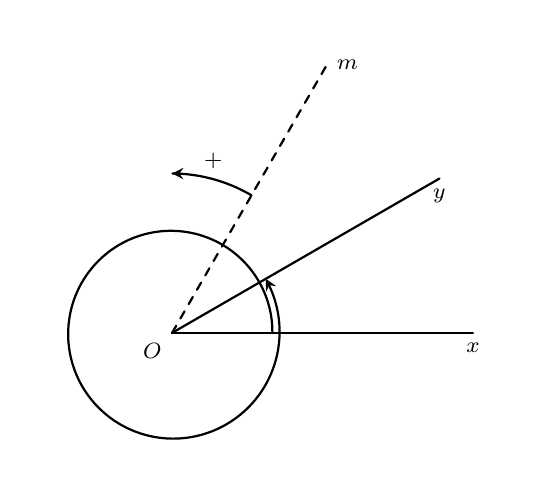
\begin{tikzpicture}[scale=1, font=\footnotesize, line join=round, line cap=round, >=stealth]
            \begin{axis}[
                axis line style={draw=none},
                axis lines=middle,
                axis equal image,
                enlargelimits,
                xtick=\empty,
                ytick=\empty,
                data cs=polar,
                samples=200,
                thick,
                line cap=round,
                line join=round,
                >=stealth
                ]
                \addplot [smooth, domain=0:390,->] {1+x/5000};
                \addplot [smooth, domain=420:450,->] {1.5+x/5000} node[above,midway]{$+$};
                \addplot [mark=none] (0.475,0) node [below left] {$O$};
                \addplot [mark=none] coordinates {(0,0) (390,3+390/5000)} node[below]{$y$};
                \addplot [mark=none] coordinates {(0,0) (0,3+0/5000)} node[below]{$x$};
                \addplot [mark=none,dashed] coordinates {(0,0) (420,3+420/5000)} node[right]{$m$};
            \end{axis}
        \end{tikzpicture}
    \end{center}
\choice
{\True $(Ox,Oy)$}
{$(Oy,Ox)$}
{$(Om,Oy)$}
{$(Om,Ox)$}
    \loigiai{
        Trong hình, góc lượng giác là $(Ox,Oy)$ với tia đầu $Ox$ và tia cuối $Oy$.
    }
    \end{ex}

\begin{ex}%[1T1B2-2]
        Cho $\tan a=\dfrac{2}{3}$, $5\pi <a<\dfrac{11\pi}{2}$. Khi đó $\cos \left(a+\dfrac{\pi}{3}\right)$ bằng
        \choice
        {$\dfrac{2\sqrt{3}+3}{2\sqrt{13}}$}
        {\True $\dfrac{2\sqrt{3}-3}{2\sqrt{13}}$}
        {$\dfrac{-2\sqrt{3}+3}{2\sqrt{13}}$}
        {$\dfrac{-2\sqrt{3}-3}{2\sqrt{13}}$}
        \loigiai{
            Ta có $\cos^2a=\dfrac{1}{1+\tan^2 a}=\dfrac{1}{1+\dfrac{4}{9}}=\dfrac{9}{13}$.\\
            Vì $5\pi <a<\dfrac{11\pi}{2}$ nên $\cos a<0$ và $\sin a<0$.\\
             Do đó, $\cos a=-\dfrac{3\sqrt{13}}{13}$ và $\sin a=-\dfrac{2\sqrt{13}}{13}$.\\
            Vậy $\cos \left(a+\dfrac{\pi}{3}\right)=\dfrac{1}{2}\cos a-\dfrac{\sqrt{3}}{2}\sin a=\dfrac{-3+2\sqrt{3}}{2\sqrt{13}}$.}
    \end{ex}

\begin{ex}%[Tex hóa SGK CD-CT,T12/22, TVN-006]%[1K1Y1-8]
    Trong các khẳng định sau, khẳng định  nào là \textbf{sai}?
    \choice
    {$\sin(\pi-\alpha)=\sin\alpha$}
    {\True $\cos(\pi-\alpha)=\cos \alpha$}
    {$\sin(\pi+\alpha)=-\sin\alpha$}
    {$\cos(\pi+\alpha)=-\cos \alpha$}
    \loigiai{
        Ta có $\cos(\pi-\alpha)=-\cos \alpha$ nên $\cos(\pi-\alpha)=\cos \alpha$ là khẳng định \textbf{sai}.
    }
\end{ex}

\begin{ex}%[1C1B1-2]
    Cho góc lượng giác gốc $O$ có tia đầu $Ou$, tia cuối $Ov$ và có số đo $\dfrac{2\pi}{3}$. Cho góc lượng giác $(O'u',O'v')$ có tia đầu $O'u'\equiv Ou$, tia cuối $O'v'\equiv Ov$. Viết công thức biểu thị số đo góc lượng giác $(O'u',O'v')$.
\choice
{$(O'u',Ov')=\dfrac{\pi}{3}+k2\pi\ (k\in \mathbb{Z})$}
{$(O'u',Ov')=\dfrac{4\pi}{3}+k2\pi\ (k\in \mathbb{Z})$}
{\True $(O'u',Ov')=\dfrac{2\pi}{3}+k2\pi\ (k\in \mathbb{Z})$}
{$(O'u',Ov')=-\dfrac{\pi}{3}+k2\pi\ (k\in \mathbb{Z})$}
    \loigiai{
        Ta có $(O'u',Ov')=(Ou,Ov)+k2\pi=\dfrac{2\pi}{3}+k2\pi\ (k\in \mathbb{Z})$.
    }
\end{ex}

\begin{ex}%[Tex hóa SGK CD-CT,T12/22, TVN-006]%[1K1B2-3]
    Rút gọn biểu thức $M=\cos(a+b)\cos(a-b)-\sin (a+b)\sin(a-b)$, ta được
    \choice
    {$M=\sin 4a$}
    {$M=1-2\cos^2a$}
    {\True $M=1-2\sin^2a$}
    {$M=\cos 4a$}
    \loigiai{
        Ta có
        \allowdisplaybreaks
        \begin{eqnarray*}
            M&=&\cos(a+b)\cos(a-b)-\sin (a+b)\sin(a-b)\\
            &=&\dfrac{1}{2}\left(\cos2a+\cos 2b\right)+\dfrac{1}{2}\left(\cos2a-\cos 2b\right)\\
            &=&\cos 2a\\
            &=&1-2\sin^2a.
        \end{eqnarray*}
    }
\end{ex}

\begin{ex}%[1T1B5-3]
        Tập nghiệm của phương trình $3\cos\left(3x-\dfrac{\pi}{3}\right)=0$ là
        \choice
        {$\left\{\dfrac{\pi}{2}+k\pi, k \in \mathbb{Z}\right\}$}
        {$\left\{\dfrac{5\pi}{6}+k 2\pi, k \in \mathbb{Z}\right\}$}
        {$\left\{\dfrac{5\pi}{18}+\dfrac{k 2\pi}{3}, k \in \mathbb{Z}\right\}$}
        {\True $\left\{\dfrac{5\pi}{18}+\dfrac{k\pi}{3}, k \in \mathbb{Z}\right\}$}
        \loigiai{
            $3\cos\left(3x-\dfrac{\pi}{3}\right)=0\Leftrightarrow 3x-\dfrac{\pi}{3}=\dfrac{\pi}{2}+k\pi\Leftrightarrow x=\dfrac{5\pi}{18}+\dfrac{k\pi}{3}, k\in\mathbb{Z}$.
            Tập nghiệm phương trình $S=\left\{\dfrac{5\pi}{18}+\dfrac{k\pi}{3}, k\in\mathbb{Z}\right\}$.
        }
    \end{ex}

\begin{ex}%[1T1B6-3]
        Phương trình $\sqrt{3}\sin x+\cos x=1$ tương đương với phương trình nào sau đây?
        \choice
        {$\cos \left( x+\dfrac{\pi}{6}\right) =\dfrac{1}{2}$}
        {$\sin \left( x+\dfrac{\pi}{3}\right) =\dfrac{1}{2}$}
        {\True $\cos \left( x-\dfrac{\pi}{3}\right) =\dfrac{1}{2}$}
        {$\sin \left( x-\dfrac{\pi}{6}\right) =\dfrac{1}{2}$}
        \loigiai{
            Chia hai vế của phương trình cho $2$, ta được
            \begin{eqnarray*}
                &\sqrt{3}\sin x+\cos x=1&\Leftrightarrow\dfrac{\sqrt{3}}{2}\sin x+\dfrac{1}{2}\cos x=\dfrac{1}{2}\\
                &&\Leftrightarrow\sin\dfrac{\pi}{3}\sin x+\cos\dfrac{\pi}{3}\cos x=\dfrac{1}{2}\\
                &&\Leftrightarrow\cos\left( x-\dfrac{\pi}{3}\right) =\dfrac{1}{2}.
            \end{eqnarray*}
        }
    \end{ex}

\begin{ex}%[1T1Y4-1]
        Tìm điều kiện xác định của hàm số  $y=\cot x$.
        \choice
        {$x \neq \dfrac{\pi}{4}+k \pi, k \in \mathbb{Z}$}
        { $x \neq k 2 \pi, k \in \mathbb{Z}$}
        {\True $x \neq k \pi, k \in \mathbb{Z}$}
        {$x\neq \dfrac{\pi}{2}+k \pi, k \in \mathbb{Z}$}
        \loigiai{
            Hàm số $y=\cot x$ xác định khi và chỉ khi $\sin x \ne 0 \Leftrightarrow x\neq k \pi, k \in \mathbb{Z} .$}
    \end{ex}

\begin{ex}%[1T1B4-2]
        Hàm số nào sau đây đồng biến trên khoảng $(0;\pi)$?
        \choice
        {\True $y=x^2$}
        {$y=\cos x$}
        {$y=\sin x$}
        {$y=\tan x$}
        \loigiai{
            Hàm số $y = x^2$ đồng biến khi $x > 0 \Rightarrow$ hàm số đồng biên trên khoảng $\left(0;\pi\right)$.}
    \end{ex}

\begin{ex}%[1C1B1-2]
    Cho góc lượng giác gốc $O$ có tia đầu $Ou$, tia cuối $Ov$ và có số đo $-\dfrac{5\pi}{6}$. Cho góc lượng giác $(O'u',O'v')$ có tia đầu $O'u'\equiv Ou$, tia cuối $O'v'\equiv Ov$. Viết công thức biểu thị số đo góc lượng giác $(O'u',O'v')$.
    \choice
    {$(O'u',Ov')=\dfrac{\pi}{6}+k2\pi\ (k\in \mathbb{Z})$}
    {$(O'u',Ov')=\dfrac{4\pi}{3}+k2\pi\ (k\in \mathbb{Z})$}
    {$(O'u',Ov')=-\dfrac{\pi}{6}+k2\pi\ (k\in \mathbb{Z})$}
    {\True $(O'u',Ov')=-\dfrac{5\pi}{6}+k2\pi\ (k\in \mathbb{Z})$}
    \loigiai{
        Ta có $(O'u',Ov')=(Ou,Ov)+k2\pi=-\dfrac{5\pi}{6}+k2\pi\ (k\in \mathbb{Z})$.
    }
\end{ex}

\begin{ex}%[1T1B4-6]
        Hình bên dưới là đồ thị của hàm số nào dưới đây?
        \begin{center}
            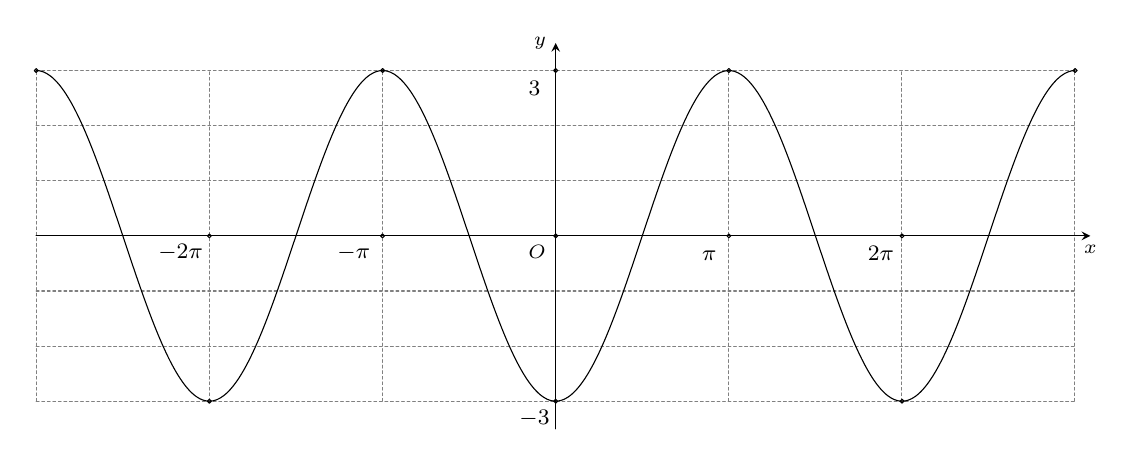
\begin{tikzpicture}[>=stealth,line join=round,line cap=round,font=\footnotesize,scale=0.7]
                \def\a{3.141592654}
                \draw[color=gray,dash pattern=on 1pt off 1pt,xstep=3.14cm,ystep=1.0cm] (-9.424,-3) grid (9.424,3);
                \draw[->] (-9.424,0) -- (9.7,0)node[below]{\scriptsize $x$};
                \draw[->] (0,-3.5) -- (0,3.5) node[left] {\scriptsize $y$};
                \draw (0,0)node[below left]{\scriptsize $O$};
                \clip (-9.58,-3.5)rectangle(9.58,3.5);
                \draw[samples=300,smooth,domain=-9.424:9.424] plot(\x,{-3*cos(\x*180/pi)});
                \path(-2*\a,0)node[shift={(-150:12pt)}]{$-2\pi$}
                (-\a,0)node[shift={(-150:12pt)}]{$-\pi$}
                (\a,0)node[shift={(-135:10pt)}]{$\pi$}
                (2*\a,0)node[shift={(-140:10pt)}]{$2\pi$}
                (0,3)node[shift={(-140:10pt)}]{$3$}
                (0,-3)node[shift={(-140:10pt)}]{$-3$};
                \foreach \x/\y in{-2*\a/0,-\a/0,\a/0,2*\a/0,-3*\a/3,3*\a/3,-2*\a/-3,2*\a/-3,\a/3,-\a/3,0/3,0/-3,0/0}\draw(\x,\y) circle (1pt);
            \end{tikzpicture}
        \end{center}
        \choice
        {\True $y=-3\cos x$}
        {$y=-2-\cos x$}
        {$y=2+|\cos x|$}
        {$y=\cos x-4$}
        \loigiai{
            \begin{itemize}
                \item $y(0)=-3\Rightarrow $ loại $y=\cos x-4$ và $y=2+|\cos x|$.
                \item $y(\pi)=3\Rightarrow $ loại $y=-2-\cos x$.
            \end{itemize}
        }
    \end{ex}

\begin{ex}%[1T1Y4-1]
        Điều kiện xác định của hàm số $y=\cot x$ là
        \choice
        { $x \ne \dfrac{\pi}{8}+k\dfrac{\pi}{2}$}
        {$x \ne \dfrac{\pi}{2}+k\pi$}
        {\True $x \ne k\pi$}
        {$x \ne \dfrac{\pi}{4}+k\pi$}
        \loigiai{
            Hàm số xác định khi và chỉ khi $\sin x \ne 0 \Leftrightarrow x \ne k\pi$, $k \in \mathbb{Z}$.
        }
    \end{ex}

\begin{ex}%[1T1B4-5]
        Cho hàm số $y=\sin^2x-\sin x+2$. Gọi $M,N$ lần lượt là GTLN và GTNN của hàm số đã cho. Khi đó $M+N$ bằng
        \choice
        {$k=-\dfrac{1}{2}$}
        {\True $\dfrac{23}{4}$}
        {$\dfrac{15}{4}$}
        {$6$}
        \loigiai{
            Ta có $y=\sin^2x-\sin x+2=\left(\sin x-\dfrac{1}{2}\right)^2+\dfrac{7}{4}$. \\
            Vì $-1 \leq \sin x \leq 1,\,\forall x \in \mathbb{R}$ nên $-\dfrac{3}{2} \leq \sin x-\dfrac{1}{2} \leq \dfrac{1}{2},\,\forall x \in \mathbb{R}$.\\
            Suy ra $0 \leq \left(\sin x-\dfrac{1}{2}\right)^2 \leq \dfrac{9}{4},\,\forall x \in \mathbb{R}$.\\
            Suy ra $\dfrac{7}{4} \leq \left(\sin x-\dfrac{1}{2}\right)^2+\dfrac{7}{4} \leq 4,\,\forall x \in \mathbb{R}$.\\
            Suy ra $\dfrac{7}{4} \leq y \leq 4,\,\forall x \in \mathbb{R}$.\\
            Vậy $M+N=\dfrac{7}{4}+4=\dfrac{23}{4}$.}
    \end{ex}

\begin{ex}%[Tex hóa SGK CD-CT,T12/22, TVN-006]%[1K1Y3-4]
    Trong các hàm số sau đây, hàm số nào là hàm tuần hoàn?
    \choice
    {$y=\tan x+x$}
    {$y=x^2+1$}
    {\True $y=\cot x$}
    {$y=\dfrac{\sin x}{x}$}
    \loigiai{
        Hàm số $y=\cot x$ là hàm số tuần hoàn với chu kỳ $T=\pi$.
    }
\end{ex}

\begin{ex}%[1T1Y1-1]
        Góc $18^\circ$ có số đo bằng rađian là bao nhiêu?
        \choice
        {$\pi$}
        {$\dfrac{\pi}{360}$}
        {\True $\dfrac{\pi}{10}$}
        {$\dfrac{\pi}{18}$}
        \loigiai{
            Ta có $18^\circ=\dfrac{\pi}{10}$ rad.
        }
    \end{ex}

\begin{ex}%[Tex hóa SGK CD-CT,T12/22, TVN-006]%[1K1Y1-4]
    Biểu diễn các góc lượng giác $\alpha=-\dfrac{5\pi}{6}$, $\beta=\dfrac{\pi}{3}$, $\gamma=\dfrac{25\pi}{3}$, $\delta=\dfrac{17\pi}{6}$ trên đường tròn lượng giác. Các góc nào có điểm biểu diễn trùng nhau?
    \choice
    {\True $\beta$ và $\gamma$}
    {$\alpha$, $\beta$, $\gamma$}
    {$\beta$, $\gamma$, $\delta$}
    {$\alpha$ và $\beta$}
    \loigiai{
        Ta có $\beta+8\pi=\dfrac{\pi}{3}+8\pi=\dfrac{25\pi}{3}=\gamma$.\\
        Do đó, $\beta$ và $\gamma$ có điểm biểu diễn trùng nhau trên đường tròn lượng giác.
    }
\end{ex}

\begin{ex}%[1C1B1-2]
    Cho góc lượng giác $(Ou,Ov)$ có số đo là $\dfrac{3\pi}{4}$, góc lượng giác $(Ou,Ow)$ có số đo là $\dfrac{5\pi}{4}$. Số đo của góc lượng giác $(Ov,Ow)$ là
\choice
{\True $(Ov,Ow)=\dfrac{\pi}{2}+k2\pi\ (k\in \mathbb{Z})$}
{$(Ov,Ow)=2\pi+k2\pi\ (k\in \mathbb{Z})$}
{$(Ov,Ow)=-\dfrac{\pi}{2}+k2\pi\ (k\in \mathbb{Z})$}
{$(Ov,Ow)=-\dfrac{\pi}{6}+k2\pi\ (k\in \mathbb{Z})$}
    \loigiai{
        Theo hệ thức Chasles, ta có
        \begin{eqnarray*}
            (Ov,Ow)&=&(Ou,Ow)-(Ou,Ov)+k2\pi\\
            &=&\dfrac{5\pi}{4}-\dfrac{3\pi}{4}+k2\pi\\
            &=&\dfrac{\pi}{2}+k2\pi\ (k\in \mathbb{Z}).
        \end{eqnarray*}
    }
\end{ex}

\begin{ex}%[1C1B1-2]
    Cho góc lượng giác gốc $O$ có tia đầu $Ou$, tia cuối $Ov$ và có số đo $45^\circ$. Cho góc lượng giác $(O'u',O'v')$ có tia đầu $O'u'\equiv Ou$, tia cuối $O'v'\equiv Ov$. Công thức biểu thị số đo góc lượng giác $(O'u',O'v')$ là
\choice
{$(O'u',Ov')=-45^\circ+k360^\circ\ (k\in \mathbb{Z})$}
{\True $(O'u',Ov')=45^\circ+k360^\circ\ (k\in \mathbb{Z})$}
{$(O'u',Ov')=135^\circ+k360^\circ\ (k\in \mathbb{Z})$}
{$(O'u',Ov')=-135^\circ+k360^\circ\ (k\in \mathbb{Z})$}
    \loigiai{
        Ta có $(O'u',Ov')=(Ou,Ov)+k360^\circ=45^\circ+k360^\circ\ (k\in \mathbb{Z})$.
    }
\end{ex}

\begin{ex}%[1T1B4-5]
        Hàm số $y=3-5\sin x$ có giá trị lớn nhất bằng
        \choice
        {$6$}
        {$2$}
        {\True $8$}
        {$4$}
        \loigiai{
            Ta có
            $$-1\le \sin x\le 1 \Leftrightarrow 5\ge-5\sin x\ge-5\Leftrightarrow  8\ge 3-5\sin x\ge -2\Rightarrow -2\le y\le 8.$$
            Suy ra giá trị lớn nhất của hàm số là $8$, đạt được khi $x=\dfrac{\pi}{2}+k2\pi,k\in\mathbb{Z}$.
        }
    \end{ex}

\begin{ex}%[1T1B2-4]
        Rút gọn biểu thức $M=\sin(\pi-a)+\tan\left(\dfrac{\pi}{2}-a\right)+\sin(-a)+\cot(\pi+a)$ được
        \choice
        {$M=2\cos a$}
        {$M=2\tan a$}
        {\True $M=2\cot a$}
        {$M=0$}
        \loigiai{
            Ta có $M=\sin a+\cot a-\sin a+\cot a=2\cot a$.
        }
    \end{ex}

\begin{ex}%[1T1Y4-6]
        Đồ thị hàm số $y=\cos x$ đi qua điểm nào sau đây?
        \choice
        {$P(-1;\pi)$}
        {$M(\pi;1)$}
        {$Q(3\pi; 1)$}
        {\True $N(0;1)$}
        \loigiai{
            Điểm $N(0;1)$ thuộc đồ thị hàm số.
        }
    \end{ex}

\begin{ex}%[1T1B4-1]
        Tập xác định của hàm số $y=2017\tan^{2018} \left( 2x+\dfrac{\pi}{3}\right)$ là
        \choice
        {\True $\mathscr{D}=\mathbb{R}\setminus\left\lbrace\dfrac{\pi}{12}+k\dfrac{\pi}{2}, k\in\mathbb{Z} \right\rbrace $}
        {$\mathscr{D}=\mathbb{R}\setminus\left\lbrace\dfrac{\pi}{2}+k\dfrac{\pi}{2}, k\in\mathbb{Z} \right\rbrace $}
        {$\mathscr{D}=\mathbb{R}\setminus\left\lbrace\dfrac{\pi}{2}+k\dfrac{\pi}{2}, k\in\mathbb{Z} \right\rbrace $}
        {$\mathscr{D}=\mathbb{R}\setminus\left\lbrace\dfrac{\pi}{2}+k\dfrac{\pi}{2}, k\in\mathbb{Z} \right\rbrace $}
        \loigiai{
            Hàm số xác định khi $2x+\dfrac{\pi}{3}\ne \dfrac{\pi}{2}+k\pi\Leftrightarrow x\ne\dfrac{\pi}{12}+k\dfrac{\pi}{2}, k\in\mathbb{Z}.$
        }
        \end{ex}

\begin{ex}%[1K1Y1-7]
        Tìm khẳng định đúng (với điều kiện các hệ thức đã xác định).
        \choice
        {$\cos \left(\pi -\alpha \right)=\cos \alpha$}
        {\True $\cos \left(-\alpha \right)=\cos \alpha$}
        {$\sin \left(\pi -\alpha \right)=-\sin \alpha$}
        {$\sin \left(-\alpha \right)=\sin \alpha$}
        \loigiai{
            Ta có
            \begin{itemize}
                \item $\sin \left(-\alpha \right)=-\sin \alpha$.
                \item $\cos \left(\pi -\alpha \right)=-\cos \alpha$.
                \item $\cos \left(-\alpha \right)=\cos \alpha$.
                \item $\sin \left(\pi -\alpha \right)=\sin \alpha$.
            \end{itemize}
        }
    \end{ex}


\noindent\textbf{II. PHẦN TỰ LUẬN:}
\begin{ex}%[Cánh Diều]%[1C1B4-3]
    Giải các phương trình
    \begin{multicols}{3}
        \begin{enumerate}[a)]
            \item $\sin x=-\dfrac{1}{2}$;
            \item $\sin x=\dfrac{\sqrt{2}}{2}$;
            \item $\sin3x=\sin2x$;
            \item $\sin x=\cos3x$;
            \item $\cos x=\dfrac{\sqrt{3}}{2}$;
            \item $\cos x=-\dfrac{\sqrt{2}}{2}$;
            \item $\cos x=-\dfrac{1}{2}$;
            \item $\cos3x=\cos\left(x+\dfrac{\pi}{3}\right)$;
            \item $\tan x=\dfrac{1}{\sqrt{3}}$;
            \item $\tan x=-1$;
            \item $\cot2x=-\sqrt{3}$.
        \end{enumerate}
    \end{multicols}
\loigiai{
\begin{enumerate}[a)]
    \item Do $\sin\left(-\dfrac{\pi}{6}\right)=-\dfrac{1}{2}$ nên $$\sin x=\sin\left(-\dfrac{\pi}{6}\right)\Leftrightarrow\hoac{&x=-\dfrac{\pi}{6}+k2\pi\\&x=\pi-\left(-\dfrac{\pi}{6}\right)+k2\pi}\Leftrightarrow\hoac{&x=-\dfrac{\pi}{6}+k2\pi\\&x=\dfrac{7\pi}{6}+k2\pi}\,(k\in\mathbb{Z}).$$
    \item Do $\sin\dfrac{\pi}{4}=\dfrac{\sqrt{2}}{2}$ nên $$\sin x=\sin\dfrac{\pi}{4}\Leftrightarrow\hoac{&x=\dfrac{\pi}{4}+k2\pi\\&x=\pi-\dfrac{\pi}{4}+k2\pi}\Leftrightarrow\hoac{&x=\dfrac{\pi}{4}+k2\pi\\&x=\dfrac{3\pi}{4}+k2\pi}\,(k\in\mathbb{Z}).$$
    \item $\sin3x=\sin2x\Leftrightarrow\hoac{&3x=2x+k2\pi\\&3x=\pi-2x+k2\pi}\Leftrightarrow\hoac{&x=k2\pi\\&x=\dfrac{\pi}{5}+k\dfrac{2\pi}{5}}\,(k\in\mathbb{Z})$.
    \item $\sin x=\cos3x\Leftrightarrow\sin x=\sin\left(\dfrac{\pi}{2}-3x\right)\Leftrightarrow\hoac{&x=\dfrac{\pi}{2}-3x+k2\pi\\&x=\pi-\left(\dfrac{\pi}{2}-3x\right)+k2\pi}\Leftrightarrow\hoac{&x=\dfrac{\pi}{8}+k\dfrac{\pi}{2}\\&x=-\dfrac{\pi}{4}+k\pi}\,(k\in\mathbb{Z})$.
    \item $\cos x=\dfrac{\sqrt{3}}{2}\Leftrightarrow\cos x=\cos\dfrac{\pi}{6}\Leftrightarrow x=\pm\dfrac{\pi}{6}+k2\pi,\,(k\in\mathbb{Z})$;
    \item $\cos x=-\dfrac{\sqrt{2}}{2}\Leftrightarrow \cos x=\cos\dfrac{3\pi}{4}\Leftrightarrow x=\pm\dfrac{3\pi}{4}+k2\pi,\,(k\in\mathbb{Z})$;
    \item $\cos x=-\dfrac{1}{2}\Leftrightarrow\cos x=\cos\dfrac{2\pi}{3}\Leftrightarrow x=\pm\dfrac{2\pi}{3}+k2\pi,\,(k\in\mathbb{Z})$;
    \item $\cos3x=\cos\left(x+\dfrac{\pi}{3}\right)\Leftrightarrow\hoac{&3x=x+\dfrac{\pi}{3}+k2\pi\\&3x=-x-\dfrac{\pi}{3}+k2\pi}\Leftrightarrow\hoac{&x=\dfrac{\pi}{6}+k\pi\\&x=-\dfrac{\pi}{12}+\dfrac{k\pi}{2}},\,(k\in\mathbb{Z})$;
    \item $\tan x=\dfrac{1}{\sqrt{3}}\Leftrightarrow\tan x=\tan\dfrac{\pi}{6}\Leftrightarrow x=\dfrac{\pi}{6}+k\pi,\,(k\in\mathbb{Z})$;
    \item $\tan x=-1\Leftrightarrow\tan x=\tan\left(-\dfrac{\pi}{4}\right)\Leftrightarrow x=-\dfrac{\pi}{4}+k\pi,\,(k\in\mathbb{Z})$;
    \item $\cot2x=-\sqrt{3}\Leftrightarrow\cot2x=\cot\left(-\dfrac{\pi}{6}\right)\Leftrightarrow x=-\dfrac{\pi}{6}+k\pi,\,(k\in\mathbb{Z})$.
\end{enumerate}}
\end{ex}

\begin{ex}%[1C1B4-3]
    Giải phương trình:
    \begin{listEX}[3]
        \item $\sin \left(2x-\dfrac{\pi}{3}\right)=-\dfrac{\sqrt{3}}{2}$;
        \item $\sin \left(3x+\dfrac{\pi}{4}\right)=-\dfrac{1}{2}$;
        \item $\cos \left(\dfrac{x}{2}+\dfrac{\pi}{4}\right) =\dfrac{\sqrt{3}}{2}$;
        \item $2\cos 3x+5=3$;
        \item $3\tan x=-\sqrt{3}$;
        \item $\cot x-3=\sqrt{3}\left(1-\cot x\right)$.
    \end{listEX}
    \loigiai{
        \begin{enumerate}[a)]
            \item Ta có 
            \begin{eqnarray*}
                &&\sin \left(2x-\dfrac{\pi}{3}\right)=-\dfrac{\sqrt{3}}{2}\\
                &\Leftrightarrow& \sin \left(2x-\dfrac{\pi}{3}\right) =\sin \left(-\dfrac{\pi}{3}\right)\\
                &\Leftrightarrow& \hoac{
                    &2x-\dfrac{\pi}{3} =-\dfrac{\pi}{3}+k2\pi\\
                    &2x-\dfrac{\pi}{3} = \pi+\dfrac{\pi}{3}+k2\pi}\\
                &\Leftrightarrow&
                \hoac{&2x=k2\pi\\&2x=\dfrac{5\pi}{3} +k2\pi}\\
                &\Leftrightarrow&
                \hoac{&x=k\pi\\ &x=\dfrac{5\pi}{6}+k\pi} (k\in \mathbb{Z}).
            \end{eqnarray*}         
            \item Ta có 
            \begin{eqnarray*}
                &&\sin \left(3x+\dfrac{\pi}{4}\right)=-\dfrac{1}{2} \\
                &\Leftrightarrow& \sin \left(3x+\dfrac{\pi}{4}\right) =\sin \left(-\dfrac{\pi}{6}\right)\\  
                &\Leftrightarrow& \hoac{
                    &3x+\dfrac{\pi}{4} = -\dfrac{\pi}{6}+k2\pi\\
                    &3x+\dfrac{\pi}{4}=\pi -\left(-\dfrac{\pi}{6}\right)+k2\pi} \\
                &\Leftrightarrow&
                \hoac{
                    &3x= -\dfrac{5\pi}{12}+k2\pi\\
                    &3x=\dfrac{11\pi}{12}+k2\pi} \\
                &\Leftrightarrow&
                \hoac{&x=-\dfrac{5}{36}+\dfrac{k2\pi}{3}\\
                    &x=\dfrac{11\pi}{36}+\dfrac{k2\pi}{3}} (k\in \mathbb{Z}).
            \end{eqnarray*}                     
            \item Ta có 
            \begin{eqnarray*}
                &&\cos \left(\dfrac{x}{2}+\dfrac{\pi}{4}\right) =\dfrac{\sqrt{3}}{2} \\ &\Leftrightarrow& \cos \left(\dfrac{x}{2}+\dfrac{\pi}{4}\right)=\cos \dfrac{\pi}{6}\\
                &\Leftrightarrow& \hoac{
                    &\dfrac{x}{2}+\dfrac{\pi}{4} = \dfrac{\pi}{6}+k2\pi\\
                    &\dfrac{x}{2}+\dfrac{\pi}{4}= -\dfrac{\pi}{6}+k2\pi}\\
                &\Leftrightarrow&
                \hoac{
                    &\dfrac{x}{2}=-\dfrac{\pi}{12}+k2\pi\\
                    &\dfrac{x}{2}=-\dfrac{5\pi}{12}+k2\pi}\\
                &\Leftrightarrow&
                \hoac{
                    &x=-\dfrac{\pi}{6}+k4\pi\\
                    &x=-\dfrac{5\pi}{6}+k4\pi} (k\in \mathbb{Z}).
            \end{eqnarray*} 
            \item Ta có $2\cos 3x+5=3 \Leftrightarrow \cos 3x =-1 \Leftrightarrow 3x=\pi+k2\pi \Leftrightarrow x = \dfrac{\pi}{3}+\dfrac{k2\pi}{3}\,\,(k\in \mathbb{Z})$.
            \item Ta có $3\tan x=-\sqrt{3} \Leftrightarrow \tan x =-\dfrac{\sqrt{3}}{3} \Leftrightarrow 
            \tan x=\tan \left(-\dfrac{\pi}{6}\right) \Leftrightarrow x=-\dfrac{\pi}{6}+k\pi\,\, (k\in \mathbb{Z}).$
            \item Ta có 
            \begin{eqnarray*}
                &&\cot x-3=\sqrt{3}\left(1-\cot x\right)\\
                &\Leftrightarrow& \cot x-3 =\sqrt{3}-\sqrt{3}\cot x\\
                &\Leftrightarrow& (1+\sqrt{3})\cot x=\sqrt{3}(1+\sqrt{3})\\
                &\Leftrightarrow& \cot x=\sqrt{3}\\
                &\Leftrightarrow& \cot x=\cot \dfrac{\pi}{6}\\
                &\Leftrightarrow& x=\dfrac{\pi}{6}+k\pi\,\, (k\in \mathbb{Z}).
            \end{eqnarray*} 
        \end{enumerate}
    }
\end{ex}

\begin{ex}%[1C1B4-3]
    Giải phương trình:
    \begin{listEX}[3]
        \item $\sin \left(2x+\dfrac{\pi}{4}\right)=\sin x$;
        \item $\sin 2x=\cos 3x$;
        \item $\cos^2 2x =\cos^2 \left(x+\dfrac{\pi}{6}\right)$.
    \end{listEX}
    \loigiai{
        \begin{enumerate}[a)]
            \item Ta có 
            \[\sin \left(2x+\dfrac{\pi}{4}\right)=\sin x
            \Leftrightarrow 
            \hoac{&2x+\dfrac{\pi}{4}=x+k2\pi\\&2x+\dfrac{\pi}{4}=\pi-x+k2\pi} 
            \Leftrightarrow \hoac{&x=-\dfrac{\pi}{4}+k2\pi\\&3x=-\dfrac{\pi}{4}+k2\pi} \Leftrightarrow \hoac{&x=-\dfrac{\pi}{4}+k2\pi\\&x=-\dfrac{\pi}{12}+\dfrac{k2\pi}{3}
            },\, (k\in \mathbb{Z}).\]
            \item Ta có 
            \begin{eqnarray*}
                \sin 2x=\cos 3x &\Leftrightarrow& \cos 3x =\cos \left(\dfrac{\pi}{2}-2x\right)\\
                &\Leftrightarrow& \hoac{
                    &3x=\dfrac{\pi}{2}-2x+k2\pi\\
                    &3x=\pi-\left(\dfrac{\pi}{2}-2x\right) +k2\pi}\\
                &\Leftrightarrow&
                \hoac{&5x=\dfrac{\pi}{2}+k2\pi\\&x=\dfrac{\pi}{2}+k2\pi}\\
                &\Leftrightarrow&
                \hoac{&x=\dfrac{\pi}{12}+\dfrac{k2\pi}{5}\\
                    &x=\dfrac{\pi}{2}+k2\pi}\, (k\in \mathbb{Z}).
            \end{eqnarray*} 
            \item Ta có $\cos^2 2x =\cos^2 \left(x+\dfrac{\pi}{6}\right) \Leftrightarrow 
            \hoac{
                &\cos 2x=\cos \left(x+\dfrac{\pi}{6}\right) &(1)\\
                &\cos 2x=-\cos \left(x+\dfrac{\pi}{6}\right). &(2)
            }$\\
            +) $(1) \Leftrightarrow \hoac{
                &2x=x+\dfrac{\pi}{6}+k2\pi\\
                &2x=-\left(x+\dfrac{\pi}{6}\right)+k2\pi
            } \Leftrightarrow
            \hoac{
                &x=\dfrac{\pi}{6}+k2\pi\\
                &3x=-\dfrac{\pi}{6}+k2\pi
            }
            \Leftrightarrow
            \hoac{
                &x=\dfrac{\pi}{6}+k2\pi\\
                &x=-\dfrac{\pi}{18}+\dfrac{k2\pi}{3}
            }(k\in \mathbb{Z})$.\\
            +) $(2) \Leftrightarrow 
            \cos 2x=\cos\left[\pi- \left(x+\dfrac{\pi}{6}\right) \right]
            \Leftrightarrow
            \hoac{
                &2x=\pi- \left(x+\dfrac{\pi}{6}\right)+k2\pi\\
                &2x=-\left[\pi- \left(x+\dfrac{\pi}{6}\right)\right]+k2\pi
            } $
            \[\Leftrightarrow
            \hoac{
                &3x=\dfrac{5\pi}{6}+k2\pi\\
                &x=-\dfrac{5\pi}{6}+k2\pi
            } \Leftrightarrow
            \hoac{
                &x=\dfrac{5\pi}{18}+\dfrac{k2\pi}{3}\\
                &x=-\dfrac{5\pi}{6}+k2\pi
            } \,(k\in\mathbb{Z}).\]
        \end{enumerate}
    }
\end{ex}

\begin{ex}Giải các phương trình sau
    \begin{listEX}[2]
        \item $2\sin x+\sqrt{2}=0$;
        \item $\sin2x-\cos x+2\sin x=1$;
        \item $3\sin ^2 x-5\sin x+2=0$;
        \item $\sqrt{3}\tan^2 x-2\tan x+\sqrt{3}=0$;
        \item $2\cos^2 2x-5\cos 2x+2=0$;
        \item $\sin^2\dfrac{x}{2}+\sin\dfrac{x}{2}-2=0$.
    \end{listEX}
    \loigiai{
        \begin{enumerate}[a)]
            \item $2\sin x+\sqrt{2}=0\Leftrightarrow\sin x=-\dfrac{\sqrt{2}}{2}\Leftrightarrow\sin x=\sin\left(-\dfrac{\pi}{4}\right)\Leftrightarrow\hoac{&x=-\dfrac{\pi}{4}+k2\pi\\&x=\dfrac{5\pi}{4}+k2\pi}\,(k\in\mathbb{Z})$;
            \item $\sin2x-\cos x+2\sin x=1\Leftrightarrow2\sin x\cos x-\cos x+2\sin x-1=0\Leftrightarrow(2\sin x-1)(\cos x+1)=0\\\Leftrightarrow\hoac{&\sin x=\dfrac{1}{2}\\&\cos x=-1}\Leftrightarrow\hoac{&\sin x=\sin\dfrac{\pi}{6}\\&x=(2k+1)\pi}\Leftrightarrow\hoac{&x=\dfrac{\pi}{6}+k2\pi\\&x=\dfrac{5\pi}{6}+k2\pi\\&x=(2k+1)\pi}\,(k\in\mathbb{Z})$;
            \item Đặt $t=\cos x$, $-1\le t\le 1$, phương trình đã cho trở thành $3t^2-5t+2=0$, ta được $t=1$ hoặc $t=\dfrac{2}{3}$.\\
            Với $t=1$ ta có $\cos x=1 \Leftrightarrow x= k2\pi,\, (k\in\mathbb{Z})$.\\
            Với $t=\dfrac{2}{3}$ ta có $\cos x=\dfrac{2}{3}=\cos\alpha\Leftrightarrow x=\pm \alpha +k2\pi,\, (k\in\mathbb{Z})$.\\
            Vậy tập nghiệm của phương trình đã cho là $S=\left\{ k2\pi, \pm \alpha+k2\pi, k\in\mathbb{Z} \right\}$.
            \item Đặt $t=\tan x$, phương trình đã cho trở thành $\sqrt{3} t^2-2t+\sqrt{3}=0$. Phương trình này vô nghiệm. Vậy phương trình đã cho vô nghiệm.
            \item $2\cos^2 2x-5\cos 2x+2=0\Leftrightarrow\hoac{&\cos2x=2\\&\cos2x=\dfrac{1}{2}}\Leftrightarrow\cos2x=\cos\dfrac{\pi}{3}\Leftrightarrow x=\pm\dfrac{\pi}{6}+k\pi,\, (k\in\mathbb{Z})$;
            \item $\sin^2\dfrac{x}{2}+\sin\dfrac{x}{2}-2=0\Leftrightarrow\hoac{&\sin\dfrac{x}{2}=1\\&\sin\dfrac{x}{2}=-2}\Leftrightarrow\dfrac{x}{2}=\dfrac{\pi}{2}+k2\pi\Leftrightarrow x=\pi+k4\pi,\, (k\in\mathbb{Z})$.
        \end{enumerate}
    }
\end{ex}

\begin{ex}%[1D1G1-5]
    Tìm giá trị lớn nhất và giá trị nhỏ nhất của hàm số  $y=2(\sin x+\cos x)+\sin 2 x+3$.
    \loigiai
    {Tập xác định $\mathscr{D}=\mathbb{R}$.\\
        Đặt $t=\sin x+ \cos x=\sqrt{2}\sin \left(x+\dfrac{\pi}{4}\right)$, $t\in \left[-\sqrt{2};\sqrt{2}\right]$.\\
        Ta có $t^2=\left(\sin x+ \cos x\right)^2=1+2\sin x\cos x=1+\sin 2x\Rightarrow \sin 2x =t^2-1$.\\
        Hàm số trở thành $y=g(t)=t^2+2t+2$. \\
        Bảng biến thiên của hàm số $y=g(t)$ trên đoạn $ \left[-\sqrt{2};\sqrt{2}\right]$
        \begin{center}
            \begin{tikzpicture}
                \tkzTabInit[lgt=1,espcl=3,deltacl=1]%nocadre,
                {$t$/1, $g(t)$ /2}
                {$-\sqrt{2}$ , $-1$ ,  $\sqrt{2}$}
                \tkzTabVar {+/$4-2\sqrt{2}$,-/$1$ ,+/ $4+2\sqrt{2}$}
            \end{tikzpicture}
        \end{center}
        Vậy $\max\limits_{x \in \mathbb{R}} y=4+2\sqrt{2}$ và $\min\limits_{x \in \mathbb{R}} y=1$.
    }
\end{ex}

\begin{ex}%[1D1K1-5]
    Tìm giá trị lớn nhất và giá trị nhỏ nhất của hàm số $y=\sqrt{3} \sin x-\cos x+5$.
    \loigiai
    {
        Tập xác định $\mathscr{D}=\mathbb{R}$.\\
        Biến đổi $y=\sqrt{3} \sin x-\cos x+5=2\left(\dfrac{\sqrt{3}}{2}\cdot\sin x-\dfrac{1}{2}\cdot\cos x\right)+5=2\sin\left(x-\dfrac{\pi}{6}\right)+5$.\\
        Với mọi $x\in \mathbb{R}$ ta có
        \allowdisplaybreaks
        \begin{eqnarray*}
            & & -1\leq \sin\left(x-\dfrac{\pi}{6}\right)\leq 1\\
            &\Leftrightarrow& -2\leq 2\sin\left(x-\dfrac{\pi}{6}\right)\leq 2\\
            &\Leftrightarrow&3\leq  2\sin\left(x-\dfrac{\pi}{6}\right)+5\leq 7.
        \end{eqnarray*}
        Vậy $\max\limits_{x \in \mathbb{R}} y=7$ khi $x=\dfrac{2\pi}{3}$ và $\min\limits_{x \in \mathbb{R}} y=3$ khi $x=-\dfrac{\pi}{3}$.
    }
\end{ex}
\Closesolutionfile{ans}